\section{Tạo bảng và dữ liệu mẫu}
\subsection{Các câu lệnh tạo bảng và ràng buộc}
Bảng Admin và Customer:
\begin{minted}{mysql}
CREATE TABLE Admin (
	AdminID        VARCHAR(9)      PRIMARY KEY,
	Username       VARCHAR(50)     NOT NULL	UNIQUE,
	Password       VARCHAR(50)     NOT NULL,
	Name           VARCHAR(50)     NOT NULL,
	Birthday       DATE            NOT NULL,
	Gender         VARCHAR(50)     NOT NULL,
	Address        VARCHAR(50)     NOT NULL,
	Phone          VARCHAR(50)     NOT NULL,
	Email          VARCHAR(50)     NOT NULL,
	Created_time   DATETIME        NOT NULL,
	Certificate    VARCHAR(10)     NOT NULL
);
\end{minted}
\begin{minted}{mysql}
CREATE TABLE Customer (
        CustomerID     VARCHAR(9)      PRIMARY KEY,
	Username       VARCHAR(50)     NOT NULL            UNIQUE,
	Password       VARCHAR(50)     NOT NULL,
	Name           VARCHAR(50)     NOT NULL,
	Birthday       DATE            NOT NULL,
	Gender         VARCHAR(50)     NOT NULL,
	Address        VARCHAR(50)     NOT NULL,
	Phone          VARCHAR(50)     NOT NULL,
	Email          VARCHAR(50)     NOT NULL,
	Created_time   DATETIME        NOT NULL,
	Total_point    BIGINT          DEFAULT(0) 
);
\end{minted}
Các bảng liên quan đến hệ thống rạp chiếu:
\begin{minted}{mysql}
CREATE TABLE Theatre (
	Branch_code    VARCHAR(2)  PRIMARY KEY,
	Name           VARCHAR(50) NOT NULL UNIQUE,
	Address        VARCHAR(50) NOT NULL
);
\end{minted}
\begin{minted}{mysql}
CREATE TABLE Room (
	Branch_code    VARCHAR(2)      REFERENCES Theatre(Branch_code)
	   ON DELETE CASCADE
	   ON UPDATE CASCADE,
	Number         INT             NOT NULL,
	State          VARCHAR(11)     NOT NULL,
	CHECK (State = 'Available' OR State = 'Unavailable'),
	PRIMARY KEY (Branch_code, Number)
);
\end{minted}
\begin{minted}{mysql}
CREATE TABLE Seat (
	Branch_code    VARCHAR(2)  NOT NULL    REFERENCES Room(Branch_code)
            ON DELETE CASCADE
            ON UPDATE CASCADE,
	Number         INT         NOT NULL    REFERENCES Room(Number)
            ON DELETE CASCADE
            ON UPDATE CASCADE,,
	Row_index      VARCHAR(1)  NOT NULL,
	Col_index      INT         NOT NULL,
	Type           VARCHAR(6)  NOT NULL,
        CHECK (Type = 'Normal' OR Type = 'VIP'),
	State          VARCHAR(11) NOT NULL, 
        CHECK (State = 'Available' OR State = 'Unavailable'), 
        PRIMARY KEY(Branch_code, Number, Row_index, Col_index)
);
\end{minted}
Bảng Movie và các bảng liên quan
\begin{minted}{mysql}
CREATE TABLE Movie (
	Movie_code     VARCHAR(9)      PRIMARY KEY,
	Director       VARCHAR(50),
	Release_date   DATE            NOT NULL,
	Age_limit      VARCHAR(3),
	Rating         DECIMAL(2,1)    CHECK (Rating > 0),
	Time_limit     DECIMAL(2,1)    CHECK (Time_limit > 0),
	Name           VARCHAR(100)    NOT NULL
);
\end{minted}
\begin{minted}{mysql}
CREATE TABLE Movie_cast (
	Movie_code     VARCHAR(50) NOT NULL    REFERENCES MOVIE(Movie_code)
            ON DELETE CASCADE
            ON UPDATE CASCADE,
	Cast           VARCHAR(50) NOT NULL,
	PRIMARY KEY (Movie_code, Cast)
);

CREATE TABLE Movie_format (
	Movie_code     VARCHAR(9)  NOT NULL    REFERENCES MOVIE(Movie_code)
            ON DELETE CASCADE
            ON UPDATE CASCADE,
	Format         VARCHAR(4)  NOT NULL,
        PRIMARY KEY (Movie_code, Format)
);

CREATE TABLE Movie_genres (
        Movie_code     VARCHAR(9)  NOT NULL    REFERENCES Movie(Movie_code)
            ON DELETE CASCADE
            ON UPDATE CASCADE,
	Genres         VARCHAR(50) NOT NULL,
        PRIMARY KEY (Movie_code, Genres)
);

CREATE TABLE Movie_language (
	Movie_code     CHAR(9)     NOT NULL    REFERENCES      Movie(Movie_code)
            ON DELETE CASCADE
            ON UPDATE CASCADE,
        Language       VARCHAR(50)		NOT NULL,
        PRIMARY KEY (Movie_code, Language)
);
\end{minted}
Bảng Movie show, Scheduled vaf bảng cOrder
\begin{minted}{mysql}
CREATE TABLE Movie_show (
        ShowID         VARCHAR(9)  PRIMARY KEY,
	Date           DATE,
	Time           FLOAT,
	AdminID        CHAR(9)    NOT NULL	REFERENCES Admin(AminID)
);

CREATE TABLE Scheduled(
        ShowID          VARCHAR(9)  NOT NULL    REFERENCES Movie_show(ShowID)
            ON DELETE CASCADE
            ON UPDATE CASCADE,,
        Branch_code     VARCHAR(2)  NOT NULL,
        Room_number     INT         NOT NULL,
        Movie_code      VARCHAR(9)  NOT NULL    REFERENCES Movie(Movie_code)
            ON DELETE CASCADE
            ON UPDATE CASCADE,,
        FOREIGN KEY (Branch_code, Room_number)      REFERENCES Room(Branch_code, Number)
            ON DELETE CASCADE
            ON UPDATE CASCADE,
        PRIMARY KEY (ShowID, Branch_code, Room_number) 
);

CREATE TABLE cOrder (
        Invoice_num     VARCHAR(9)     NOT NULL    PRIMARY KEY,
        Pay_time        DATETIME       NOT NULL,
        Total_price     FLOAT          NOT NULL,
        CustomerID      VARCHAR(9)     NOT NULL,
        FOREIGN KEY (CustomerID)       REFERENCES Customer(CustomerID)
);
\end{minted}
Bảng Food và Food\_order
\begin{minted}{mysql}
CREATE TABLE Food (
        FoodID          VARCHAR(2)  PRIMARY KEY,
        Name            VARCHAR(7)  NOT NULL,
        Size            VARCHAR(1)  NOT NULL
);

CREATE TABLE Food_order (
        FoodID          VARCHAR(2)    NOT NULL,
        Invoice_num     VARCHAR(50)   NOT NULL,
        Amount          INT           NOT NULL,
        FOREIGN KEY (FoodID) REFERENCES Food(FoodID)
            ON UPDATE CASCADE,
        FOREIGN KEY (Invoice_num) REFERENCES cOrder(Invoice_num)
            ON DELETE CASCADE
            ON UPDATE CASCADE,
        PRIMARY KEY (FoodID, Invoice_num) 
);
\end{minted}
Bảng Ticket, Voucher và isApplied
\begin{minted}{mysql}
CREATE TABLE Ticket (
	TicketID           VARCHAR(9)  NOT NULL 	PRIMARY KEY,
	Invoice_num        VARCHAR(9)  NOT NULL 	REFERENCES cOrder(Invoice_num)
            ON DELETE CASCADE
            ON UPDATE CASCADE,
	Branch_code        VARCHAR(2)  NOT NULL,
	Room_number        INT         NOT NULL,
	Row_index          VARCHAR(1)  NOT NULL,
	Col_index          INT         NOT NULL,
        ShowID             VARCHAR(9)  NOT NULL 	REFERENCES MOVIE_SHOW(ShowID)
            ON UPDATE CASCADE,
        FOREIGN KEY (Branch_code, Room_number, Row_index, Col_index) 
	REFERENCES Seat(Branch_code, Number, Row_index, Col_index)
);
\end{minted}
\begin{minted}{mysql}
CREATE TABLE Voucher (
	VoucherID          VARCHAR(9)      PRIMARY KEY,
	S_time             DATETIME        NOT NULL,
 	E_time            DATETIME        NOT NULL,
	Gender             VARCHAR(20),
	Order_price        INT,
	Total_point        INT             CHECK (Total_point >= 0),
	Description        VARCHAR(100)    NOT NULL,
	Discount_percent   INT             NOT NULL
);

CREATE TABLE isApplied (
	VoucherID          VARCHAR(9)	NOT NULL REFERENCES Voucher(VoucherID)
            ON UPDATE CASCADE,
	Invoice_num        VARCHAR(9)	NOT NULL REFERENCES cOrder(Invoice_num)
            ON UPDATE CASCADE,
	PRIMARY KEY (VoucherID, Invoice_num)
);
\end{minted}
\subsection{Các câu lệnh INSERT dữ liệu}
Thêm dữ liêu vào bảng Admin:
\begin{minted}{mysql}
    INSERT INTO Admin (AdminID, Username, Password, Name, Birthday, Gender, Address, Phone, Email, Created_time, Certificate) VALUES ('a85604932', 'acaustic0', 'qvtvFVlxRb', 'Arda Caustic', '1920-11-13', 'Female', '581 Moland Way', '0359168412', 'acaustic0@fda.gov', '2022-07-07 8:59', 'Sales');
\end{minted}
Thêm dữ liêu vào bảng Customer:
\begin{minted}{mysql}
    INSERT INTO Customer (CustomerID, Username, Password, Name, Birthday, Gender, Address, Phone, Email, Created_time, Total_point) VALUES ('c00440411', 'cjohansenct', '23QWR0mat0WD', 'Courtnay Johansen', '1977-06-18', 'Other', '33450 Division Park', '0749066144', 'cjohansenct@netscape.com', '2021-08-05 11:50:00', 170);
\end{minted}
Thêm dữ liêu vào bảng Theatre:
\begin{minted}{mysql}
    INSERT INTO Theatre (Branch_code, Name, Address) values ('b0', 'CGV Sinh viên', '71100 Swallow Street');
    INSERT INTO Theatre (Branch_code, Name, Address) values ('b1', 'CGV Vincom Bách Khoa', '857 Lunder Drive');
\end{minted}
Thêm dữ liêu vào bảng Room:
\begin{minted}{mysql}
    INSERT INTO Room (Branch_code, Number, State) values ('b0', 1, 'Available');
    INSERT INTO Room (Branch_code, Number, State) values ('b0', 2, 'Unavailable');
    INSERT INTO Room (Branch_code, Number, State) values ('b0', 3, 'Available');
    INSERT INTO Room (Branch_code, Number, State) values ('b0', 4, 'Available');
    INSERT INTO Room (Branch_code, Number, State) values ('b0', 5, 'Unavailable');
\end{minted}
Thêm dữ liêu vào bảng Seat:
\begin{minted}{mysql}
    INSERT INTO Seat (Branch_code, Number, Row_index, Col_index, Type, State) VALUES ('b0', 1, 'A', 1, 'Normal', 'Available');
    INSERT INTO Seat (Branch_code, Number, Row_index, Col_index, Type, State) VALUES ('b0', 1, 'A', 2, 'Normal', 'Available');
\end{minted}
Thêm dữ liêu vào bảng Movie:
\begin{minted}{mysql}
    INSERT INTO Movie (Movie_code, Director, Release_date, Age_limit, Rating,Time_limit, Name) VALUES ('m55319663','Simmonds Sallings','2019-12-31','All',1.4,1.6,'The Shawshank Redemption ');
\end{minted}
Thêm dữ liêu vào bảng Movie\_cast:
\begin{minted}{mysql}
    INSERT INTO Movie_cast (Movie_code, Cast) VALUES ('m55319663', 'Edita Castiblanco');
    INSERT INTO Movie_cast (Movie_code, Cast) VALUES ('m84499891', 'Dame End');
    INSERT INTO Movie_cast (Movie_code, Cast) VALUES ('m64267580', 'Amos Jore');
    INSERT INTO Movie_cast (Movie_code, Cast) VALUES ('m12968902', 'Cirillo Ridde');
    INSERT INTO Movie_cast (Movie_code, Cast) VALUES ('m04905601', 'Cara Barthod');
\end{minted}
Thêm dữ liêu vào bảng Movie\_format:
\begin{minted}{mysql}
    INSERT INTO Movie_format (Movie_code, Format) VALUES ('m00036050', '2D');
    INSERT INTO Movie_format (Movie_code, Format) VALUES ('m00036050', '3D');
    INSERT INTO Movie_format (Movie_code, Format) VALUES ('m00036050', '4DX');
    INSERT INTO Movie_format (Movie_code, Format) VALUES ('m00036050', 'IMAX');
    INSERT INTO Movie_format (Movie_code, Format) VALUES ('m01089002', '2D');
\end{minted}

Thêm dữ liêu vào bảng Movie\_genres:
\begin{minted}{mysql}
    INSERT INTO Movie_genres (Movie_code, Genres) VALUES ('m00036050', 'Crime');
    INSERT INTO Movie_genres (Movie_code, Genres) VALUES ('m00036050', 'Musical');
    INSERT INTO Movie_genres (Movie_code, Genres) VALUES ('m01089002', 'Action');
    INSERT INTO Movie_genres (Movie_code, Genres) VALUES ('m01089002', 'Western');
    INSERT INTO Movie_genres (Movie_code, Genres) VALUES ('m01811816', 'Crime');
\end{minted}

Thêm dữ liêu vào bảng Movie\_language:
\begin{minted}{mysql}
    INSERT INTO Movie_language (Movie_code, Language) VALUES ('m00036050', 'Finnish');
    INSERT INTO Movie_language (Movie_code, Language) VALUES ('m00036050', 'Kurdish');
    INSERT INTO Movie_language (Movie_code, Language) VALUES ('m01089002', 'Hungarian');
    INSERT INTO Movie_language (Movie_code, Language) VALUES ('m01089002', 'Tetum');
    INSERT INTO Movie_language (Movie_code, Language) VALUES ('m01811816', 'Gujarati');
\end{minted}

Thêm dữ liêu vào bảng Movie\_show:
\begin{minted}{mysql}
    INSERT INTO Movie_show (ShowID, Date, Time, AdminID) VALUES ('s82663010', '2022-01-24', 20, 'a85604932');
    INSERT INTO Movie_show (ShowID, Date, Time, AdminID) VALUES ('s97179598', '2022-01-02', 12, 'a29746909');
\end{minted}

Thêm dữ liêu vào bảng Scheduled:
\begin{minted}{mysql}
    INSERT INTO Scheduled (ShowID, Branch_code, Room_number, Movie_code) VALUES ('s82663010', 'b0', 1, 'm55319663');
    INSERT INTO Scheduled (ShowID, Branch_code, Room_number, Movie_code) VALUES ('s97179598', 'b0', 2, 'm84499891');
\end{minted}

Thêm dữ liêu vào bảng cOrder:
\begin{minted}{mysql}
    INSERT INTO cOrder (Invoice_num, Pay_time, Total_price, CustomerID) VALUES ('o00128357', '2021-10-10 3:17', 1600000, 'c80888111');
    INSERT INTO cOrder (Invoice_num, Pay_time, Total_price, CustomerID) VALUES ('o00266088', '2020-12-27 6:47', 2700000, 'c07619154');
\end{minted}

Thêm dữ liêu vào bảng Food:
\begin{minted}{mysql}
    INSERT INTO Food (FoodID, Name, Size) values ('f0', 'Popcorn', 'S');
    INSERT INTO Food (FoodID, Name, Size) values ('f1', 'Popcorn', 'M');
    INSERT INTO Food (FoodID, Name, Size) values ('f2', 'Popcorn', 'L');
    INSERT INTO Food (FoodID, Name, Size) values ('f3', 'Pepsi', 'S');
    INSERT INTO Food (FoodID, Name, Size) values ('f4', 'Pepsi', 'M');
\end{minted}

Thêm dữ liêu vào bảng Food\_order:
\begin{minted}{mysql}
    INSERT INTO Food_order (FoodID, Invoice_num, Amount) VALUES ('f8', 'o00128357', 4);
    INSERT INTO Food_order (FoodID, Invoice_num, Amount) VALUES ('f8', 'o00266088', 2);
    INSERT INTO Food_order (FoodID, Invoice_num, Amount) VALUES ('f7', 'o00325858', 4);
    INSERT INTO Food_order (FoodID, Invoice_num, Amount) VALUES ('f3', 'o00594733', 1);
    INSERT INTO Food_order (FoodID, Invoice_num, Amount) VALUES ('f3', 'o00868179', 2);
\end{minted}

Thêm dữ liêu vào bảng Ticket:
\begin{minted}{mysql}
    INSERT INTO Ticket (TicketID, Invoice_num, Branch_code, Room_number, Row_index, Col_index, ShowID) VALUES ('t00395523', 'o00128357', 'b0', 1, 'A', 1, 's82663010');
    INSERT INTO Ticket (TicketID, Invoice_num, Branch_code, Room_number, Row_index, Col_index, ShowID) VALUES ('t00422454', 'o00266088', 'b0', 1, 'A', 2, 's82663010');
\end{minted}

Thêm dữ liêu vào bảng Voucher:
\begin{minted}{mysql}
    INSERT INTO Voucher (VoucherID, S_time, E_time, Gender, Order_price ,Total_point, Description, Discount_percent) VALUES ('v55009817','2022-12-17 10:13','2022-12-31 6:21','Male',4000000,470,'Martin Luther King Day',45);
    INSERT INTO Voucher (VoucherID, S_time, E_time, Gender, Order_price ,Total_point, Description, Discount_percent) VALUES ('v66199029','2022-12-20 18:55','2022-12-21 11:18','Non-binary',6400000,760,'Presidents\' Day',35);

\end{minted}

Thêm dữ liêu vào bảng isApplied:
\begin{minted}{mysql}
    INSERT INTO isApplied(VoucherID, Invoice_num) VALUES('v55009817', 'o00128357');
    INSERT INTO isApplied(VoucherID, Invoice_num) VALUES('v66199029', 'o00266088');
    INSERT INTO isApplied(VoucherID, Invoice_num) VALUES('v98346309', 'o00325858');
    INSERT INTO isApplied(VoucherID, Invoice_num) VALUES('v11176701', 'o00594733');
    INSERT INTO isApplied(VoucherID, Invoice_num) VALUES('v47527039', 'o00868179');
\end{minted}

\subsection{Kết quả dữ liệu từ các bảng}
\begin{figure}[H]
    \centering
    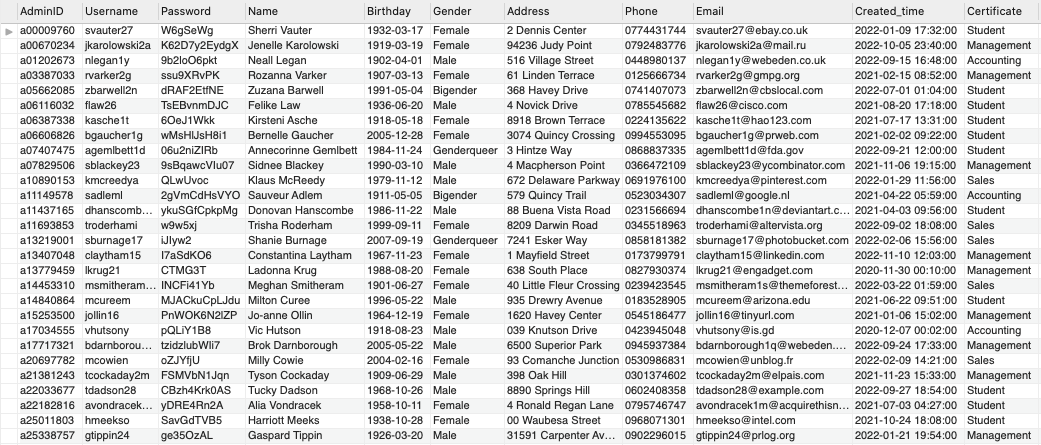
\includegraphics[width=\textwidth]{images/ADMIN.png}
    \caption{Bảng Admin}
\end{figure}

\begin{figure}[H]
    \centering
    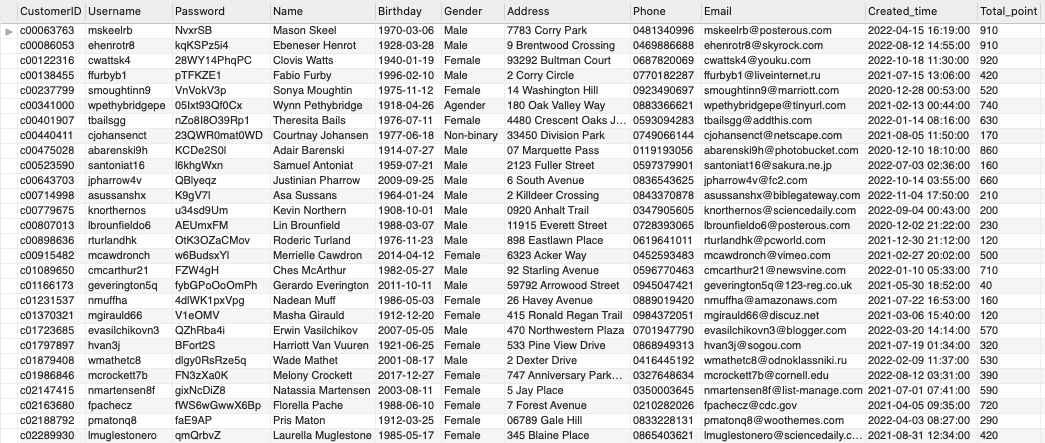
\includegraphics[width=\textwidth]{images/CUSTOMER.png}
    \caption{Bảng Customer}
\end{figure}

\begin{figure}[H]
    \centering
    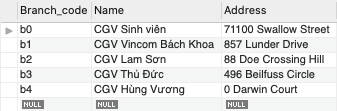
\includegraphics[width=10cm]{images/THATRE.png}
    \caption{Bảng Theatre}
\end{figure}

\begin{figure}[H]
    \centering
    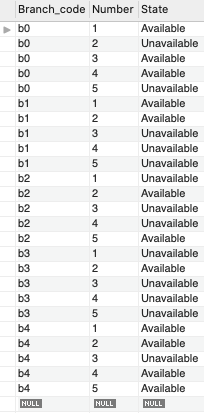
\includegraphics[width=5cm]{images/ROOM.png}
    \caption{Bảng Room}
\end{figure}

\begin{figure}[H]
    \centering
    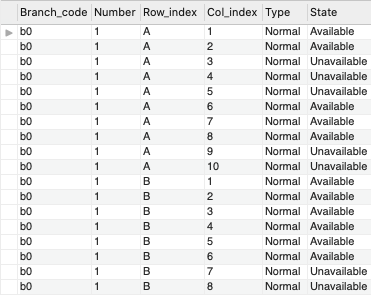
\includegraphics[width=10cm]{images/SEAT.png}
    \caption{Bảng Seat}
\end{figure}

\begin{figure}[H]
    \centering
    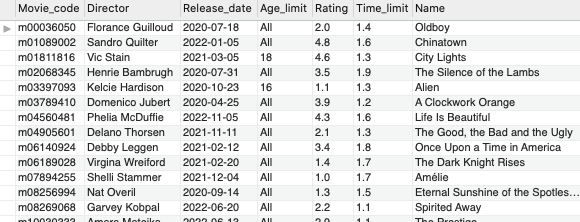
\includegraphics[width=\textwidth]{images/MOVIE.png}
    \caption{Bảng Movie}
\end{figure}

\begin{figure}[H]
    \centering
    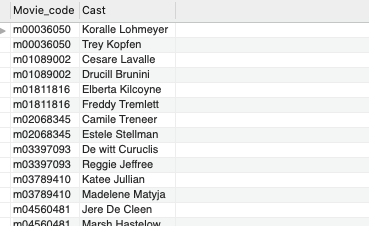
\includegraphics[width=10cm]{images/CAST.png}
    \caption{Bảng Movie\_cast}
\end{figure}

\begin{figure}[H]
\begin{subfigure}{.5\textwidth}
  \centering
  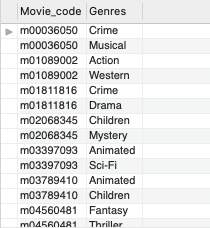
\includegraphics[width=.8\linewidth]{images/GENRES.png}
\end{subfigure}%
\begin{subfigure}{.5\textwidth}
  \centering
  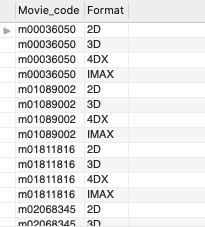
\includegraphics[width=.8\linewidth]{images/FORMAT.png}
\end{subfigure}
\caption{Bảng Movie\_genres và Movie\_format}
\end{figure}

\begin{figure}[H]
\begin{subfigure}{.5\textwidth}
  \centering
  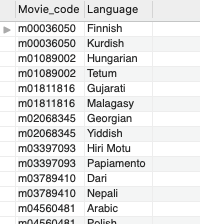
\includegraphics[width=.8\linewidth]{images/LANGUAGE.png}
\end{subfigure}%
\begin{subfigure}{.5\textwidth}
  \centering
  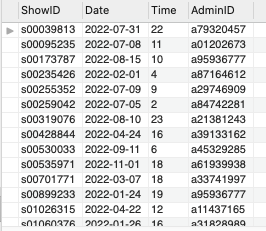
\includegraphics[width=.8\linewidth]{images/MOVIE_SHOW.png}
\end{subfigure}
\caption{Bảng Movie\_language và Movie\_show}
\end{figure}

\begin{figure}[H]
    \centering
    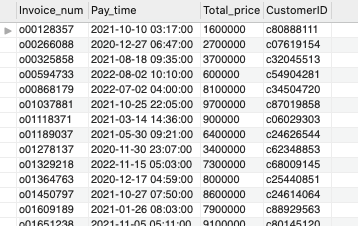
\includegraphics[width=12cm]{images/ORDER.png}
    \caption{Bảng cOrder}
\end{figure}

\begin{figure}[H]
\begin{subfigure}{.5\textwidth}
  \centering
  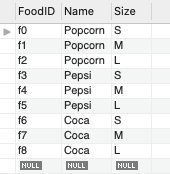
\includegraphics[width=.8\linewidth]{images/FOOD.png}
\end{subfigure}%
\begin{subfigure}{.5\textwidth}
  \centering
  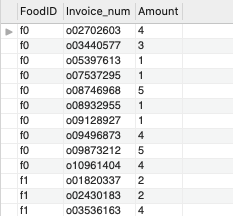
\includegraphics[width=.8\linewidth]{images/FOOD_ORDER.png}
\end{subfigure}
\caption{Bảng Food và Food\_order}
\end{figure}

\begin{figure}[H]
    \centering
    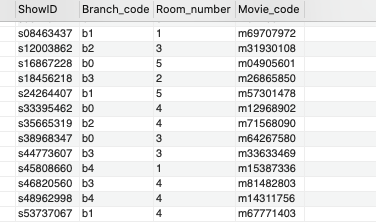
\includegraphics[width=12cm]{images/SCHEDULED.png}
    \caption{Bảng Scheduled}
\end{figure}

\begin{figure}[H]
    \centering
    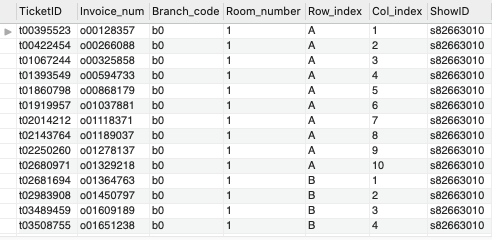
\includegraphics[width=12cm]{images/TICKET.png}
    \caption{Bảng Ticket}
\end{figure}

\begin{figure}[H]
    \centering
    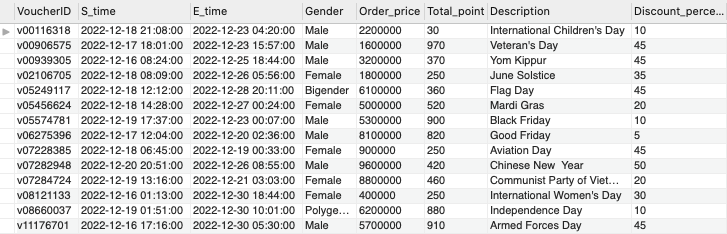
\includegraphics[width=15cm]{images/VOUCHER.png}
    \caption{Bảng Voucher}
\end{figure}

\begin{figure}[H]
    \centering
    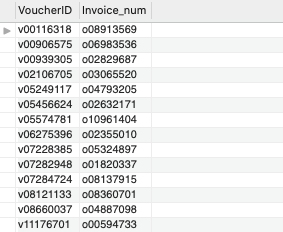
\includegraphics[width=10cm]{images/IS_APPLIED.png}
    \caption{Bảng isApplied}
\end{figure}

